\documentclass[11pt,a4paper]{article}
\usepackage[top=3cm, bottom=2cm, left=2cm, right=2cm]{geometry}
\usepackage[utf8]{inputenc}
\usepackage{amsmath, amsfonts, amssymb}
\usepackage{siunitx}
\usepackage[brazil]{babel}
\usepackage{graphicx}
\usepackage[margin=10pt,font={small, it},labelfont=bf, textfont=it]{caption}
\usepackage[dvipsnames, svgnames]{xcolor}
\DeclareCaptionFont{MediumOrchid}{\color[svgnames]{MediumOrchid}}
\usepackage[pdftex]{hyperref}
\usepackage{natbib}
\bibliographystyle{plainnat}
\bibpunct{[}{]}{,}{s}{}{}
\usepackage{color}
\usepackage{footnote}
\usepackage{setspace}
\usepackage{booktabs}
\usepackage{multirow}
\usepackage{subfigure}
\usepackage{fancyhdr}
\usepackage{leading}
\usepackage{indentfirst}
\usepackage{wrapfig}
\usepackage{mdframed}
\usepackage{etoolbox}
\usepackage[version=4]{mhchem}
\usepackage{enumitem}
\usepackage{caption}
\usepackage{titlesec}
\usepackage{tcolorbox}
\usepackage{tikz}
\usepackage{LobsterTwo}
\usepackage[T1]{fontenc}
\usepackage{fontspec}
\usepackage{txfonts}
\AtBeginEnvironment{equation}{\fontsize{13}{16}\selectfont}


\titleformat{\section}{\LobsterTwo\LARGE\color{CarnationPink}}{\thesection.}{1em}{}
\titleformat{\subsection}{\LobsterTwo\LARGE\color{CarnationPink}}{\thesubsection}{1em}{}


\DeclareCaptionLabelFormat{figuras}{\textcolor{DarkTurquoise}{Figura \arabic{figure}}}
\captionsetup[figure]{labelformat=figuras}

\makeatletter
\renewcommand\tagform@[1]{\maketag@@@{\color{CarnationPink}(#1)}}
\makeatother

\renewcommand{\theequation}{Eq. \arabic{equation}}
\renewcommand{\thefigure}{Fig. \arabic{figure}}
\renewcommand{\thesection}{\textcolor{CarnationPink}{\arabic{section}}}

\setlist[itemize]{label=\textcolor{CarnationPink}{$\mathbf{\square}$}}

\setlist[enumerate]{label=\textcolor{CarnationPink}{\arabic*.}, align=left}


\newcounter{exemplo}

\NewDocumentEnvironment{exemplo}{ O{} }{%
\allowbreak
\setlength{\parindent}{0pt}
  \begin{mdframed}[
  leftline=true,
  topline=false,
  rightline=false,
  bottomline=false,
  linewidth=2pt,
  linecolor=CarnationPink,
  frametitlerule=false,
  frametitlefont=\LobsterTwo\large\color{CarnationPink},
  frametitle={\color{CarnationPink}\LobsterTwo\large #1},
  ]
}{%
  \end{mdframed}
}

\setlength{\fboxsep}{5pt}
\setlength{\fboxrule}{1.5pt}
\usepackage{float}
\renewcommand{\thefootnote}{\alph{footnote}}
\usepackage{url}
\hypersetup{
	colorlinks=true,
	linkcolor=DarkTurquoise,
	filecolor=DarkTurquoise,      
	urlcolor=DarkTurquoise,
	citecolor=DarkTurquoise,
	pdftitle={Especialista em Física da Radioterapia}
}
\pagestyle{fancy}
\fancyhf{}
\renewcommand{\headrulewidth}{0pt}
\rfoot{Página \thepage}

\title{\LobsterTwo\Huge{Braquiterapia}}
\author{\LobsterTwo\Large{Braquiterapia Intersticial}\nocite{*}}
\date{\LobsterTwo\textit{Dalila Mendonça}}
\begin{document}
	\maketitle

\section{Introdução}

	A braquiterapia intersticial tem uma longa tradição, começando com agulhas de rádio sendo implantadas em tumores superficiais na década de 1930. Os sistemas de implantes desenvolvidos na época, Manchester e Quimby, ainda orientam os padrões de inserção de agulhas utilizados em implantes atualmente.

	Embora as agulhas de rádio tenham sido inicialmente usadas para implantes intersticiais, outros núcleos radioativos foram desenvolvidos ao longo do tempo. As fitas de baixa taxa de dose (LDR) de \ce{^{192}Ir} ou \ce{^{137}Cs} foram os dispositivos mais populares para braquiterapia intersticial até que afterloaders remotos de alta taxa de dose (HDR) foram desenvolvidos. Em comparação com a braquiterapia LDR, os afterloaders HDR reduzem a exposição dos médicos e da equipe que está tratando o paciente, reduzem o tempo que o paciente permanece internado e permitem mais flexibilidade na personalização dos planos de tratamento. Além disso, o número de fontes que precisam ser mantidas, calibradas e armazenadas com segurança é significativamente reduzido em HDR em comparação com LDR.

	A transição da LDR para a HDR levantou algumas preocupações com respeito a mudança na morte celular devido a0 diferença radiobiologica entre os dois métodos. Portanto, alguns centros desenvolveram um método de entrega de taxa de dose pulsada (PDR) para a transição dos métodos, no qual os afterloaders HDR foram utilizados para entregar frações da dose total (pulsos de dose) em intervalos de tempo predefinidos, normalmente de 1 hora. À medida que os dados dos resultados e a toxicidade da Braquiterapia Intersticial HDR amadureceram, os tratamentos de PDR e  LDR estão caindo em desuso.

	A braquiterapia intersticial pode ser usada como terapia exclusiva ou como terapia adjuvante (boost) à teleterapia. Sua principal característica é a administração de doses altamente conformadas com gradientes de dose acentuados em tumores que não são ressecáveis cirurgicamente devido à proximidade de órgãos de risco. A braquiterapia intersticial também pode ser usada em pacientes que não são candidatos à cirurgia. Essas vantagens devem ser cuidadosamente ponderadas em relação aos riscos inertes do procedimento, incluindo o risco da anestesia local, infecção e a imobilização do paciente durante o tratamento.

\section{Sítios de Tratamento}

\subsection*{Ginecológicos}

	A doença em estágio inicial às vezes é tratada com implantes intracavitários (por exemplo, tandem e ovoide); A braquiterapia intersticial para o tratamento do câncer de colo de útero é usada como último recurso caso o tratamento com o feixe externo não consiga reduzir o tamanho do tumor suficientemente de modo que seja possível obter uma cobertura satisfatória com um implante intracavitário. Existem várias opções para a concepção do implante intersticial, incluindo aqueles que são uma combinação de componentes intracavitários e intersticiais:
	
	\begin{itemize}[label=\textcolor{CarnationPink}{$\star$}]
		\item Tandem e anel (T\&R)/tandem e ovoide (T\&O) com duas a três agulhas intersticiais manuais;
		\item Aplicadores T\&O  combinados com canais intersticiais;
		\item Implante perineal com cilindro vaginal central, modelo de cateter em tandem e disposto concentricamente. Um aplicador comum é o template Syed-Neblett (\ref{fig:syed}), que consiste em 12 cateteres intersticiais ao redor de um cilindro central, embora outros aplicadores estejam disponíveis.
	\end{itemize}

	\begin{figure}[h]
		\centering
		\subfigure{
			\fcolorbox{DarkTurquoise}{white}{%
				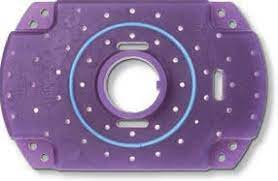
\includegraphics[width=0.36\textwidth]{Imagens/syed1.jpg}
			}} %
			\subfigure{
			\fcolorbox{DarkTurquoise}{white}{%
				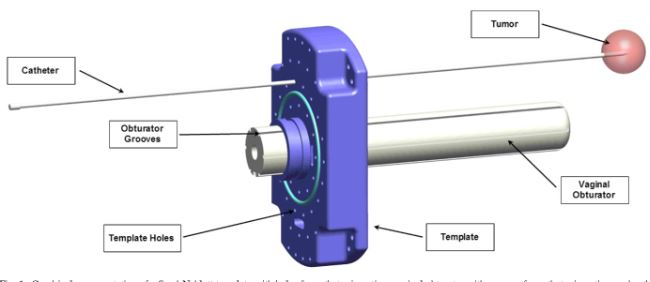
\includegraphics[width=0.54\textwidth]{Imagens/syed2.JPG}
			}} %
		\caption{Template Syed-Neblett para braquiterapia intracavitária ginecológica.}
		\label{fig:syed}
	\end{figure} 

	Embora seja mais invasivo, estudos de planejamento sugerem uma melhor cobertura com o template Syed-Neblett. Uma variedade de esquemas de dose e fracionamento são utilizados na braquiterapia intersticial para cânceres ginecológicos, variando de 1 a 8 frações, diariamente ou duas vezes ao dia (BID), normalmente até uma dose biologicamente ponderada de 75 a 85 Gy (BED).

	Para câncer vaginal, os guidelines da American Brachytherapy Society (ABS) para braquiterapia intersticial para câncer vaginal recomendam que pacientes com doença volumosa (bulky) ($\geq$ 0.5 cm) sejam considerados para tratamentos com implantes intersticiais. Devido à raridade da doença, os guidelines são baseados nos resultados de estudos de uma única instituição, uma vez que não há dados de trials prospectivos randomizados disponíveis atualmente. Um modelo de implante perineal cilindricamente simétrico com um cilindro vaginal é o mais indicado para este tipo de implante. O espaçamento típico entre as agulhas normalmente não é superior a 1 cm. Os esquemas de fracionamento de dose incluem 2 Gy x 18 frações de teleterapia (EBRT) seguidas de 6 Gy x 5 frações de braquiterapia ou  1.8 Gy x 28 frações de EBRT seguidas de 7 Gy x 3 frações de braquiterapia.

\subsection*{Mama}

	O objetivo da braquiterapia intersticial da mama é fornecer irradiação parcial acelerada da mama (APBI) na cavidade da mastectomia após a cirurgia. Os tratamentos de mama intersticial se enquadram em duas categorias:

	\begin{enumerate}
		\item HDR intersticial usando dois planos de agulhas implantadas; e
		\item Braquiterapia HDR parcial da mama com aplicadores implantados na cavidade cirúrgica.
		\item Obs: A radioterapia intraoperatória (IORT) também pode utilizar braquiterapia HDR para tratamentos de mama ;
	\end{enumerate}

	\begin{wrapfigure}{L}{0.4\textwidth}
		\centering
		\fcolorbox{DarkTurquoise}{white}{%
			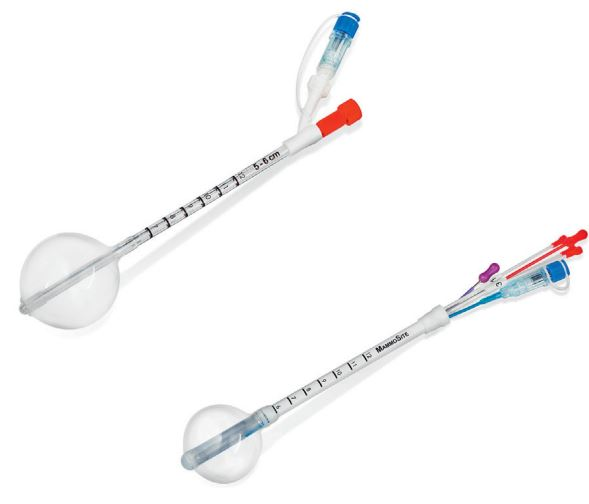
\includegraphics[width=0.35\textwidth]{Imagens/mamosite.JPG}
		}%
		\caption{Aplicador MammoSite}
		\label{fig:mamosite}
	\end{wrapfigure}

	Uma variedade de aplicadores foram desenvolvidos para inserção na cavidade da mastectomia. O dispositivo MammoSite (mostrado na \ref{fig:mamosite}) possui vários tamanhos de aplicadores  pressurizados (por exemplo, esferas de 4-5 cm e 5-6 cm de diâmetro; e um elipsóide de 4 cm x 6 cm), que é preenchido com solução salina. Um cateter de silicone está localizado no centro do balão. O objetivo do balão é moldar o tecido da cavidade da mastectomia em uma forma esférica, que pode então ser irradiada. O implante do aplicador de balão pode ser feito no momento da cirurgia ou logo após. Idealmente, deve haver alguns dias de espera entre o implante e a imagem para o planejamento do tratamento para permitir que as bolsas de ar se resolvam e o seroma\footnote{Um seroma é uma coleção de fluido seroso, que é um líquido amarelado e transparente produzido pelo organismo que normalmente ocorre como resultado de um procedimento cirúrgico ou de um trauma, quando o tecido é danificado e ocorre acúmulo de fluido no local da lesão. } seja drenado.

	Um fator limitante para os tratamentos originais do aplicador MammoSite é a proximidade da cavidade da lumpectomia com a pele do paciente. São necessários pelo menos 7 mm de espaçamento para evitar potencial toxicidade tardia com um resultado cosmético insatisfatório. Para superar o problema de economia de pele, vários cateteres multilúmen foram desenvolvidos para permitir a modelagem de dose assimétrica para melhorar a economia de pele. Estes incluem cateteres de balão multilúmen, bem como cateteres multilúmen sem o uso de um balão (por exemplo, o aplicador SAVI apresentado na \ref{fig:savi}).

	\begin{wrapfigure}{R}{0.4\textwidth}
		\centering
		\fcolorbox{DarkTurquoise}{white}{%
			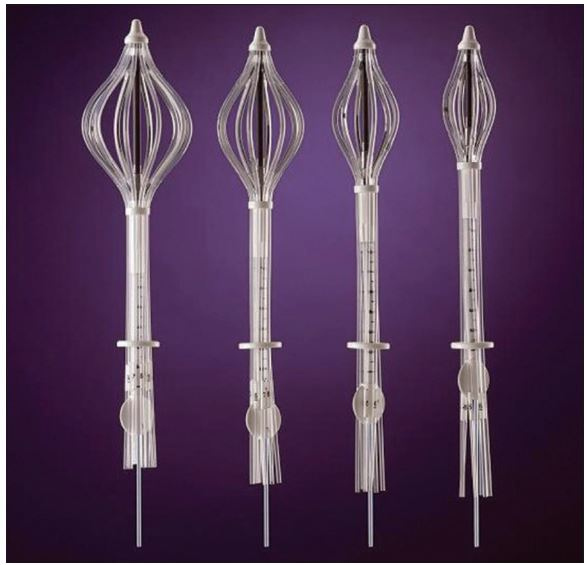
\includegraphics[width=0.35\textwidth]{Imagens/savi.JPG}
		}%
		\caption{Aplicador SAVI}
		\label{fig:savi}
	\end{wrapfigure}

	Os implantes mamários intersticiais com cateteres são utilizados se a cavidade da mastectomia for muito pequena para o implante de outros aplicadores ou se a cavidade tiver fechado antes da implantação do aplicador. Normalmente, são colocados de 10 a 20 cateteres em um arranjo plano através da região do tumor. O regime de tratamento é semelhante aos tratamentos de cavidade tumoral (ou seja, uma semana de 10 frações administradas em BID). Para minimizar a exposição desnecessária do paciente à radiação especialmente a mama contralateral, é importante colocar os cateteres de forma que as pontas dos cateteres estejam localizadas na linha média do paciente.

	Além dessas técnicas, a IORT pode ser utilizada para fornecer um boost ao local da mastectomia no momento da cirurgia. Isso é apoiado pelos resultados de 5 anos recentemente relatados do estudo TARGIT-A. Os principais sistemas em uso para IORT são o dispositivo Zeiss Intrabeam, um alvo de baixo kV e aplicador em um braço móvel, e o sistema Xoft/Axxent, um tubo de raios X de baixo kV em um cateter que é usado em combinação com um aplicador de balão. Devido à semelhança na energia do feixe desses dispositivos com as fontes tradicionais de braquiterapia, eles são frequentemente classificados como “braquiterapia eletrônica”. O AAPM TG-182 fornece recomendações para o controle de qualidade em braquiterapia eletrônica.

	Os esquemas de fracionamento de dose publicados para a maioria dos alvos intersticiais dependem da experiência de estudos relativamente pequenos de uma única instituição. A exceção notável são os tratamentos intersticiais para a mama, que seguem um protocolo APBI muito bem definido. Os constraints de dose estão listados na \ref{fig:constraintsApbi}.

	\begin{figure}[h]
		\centering
		\fcolorbox{DarkTurquoise}{white}{%
			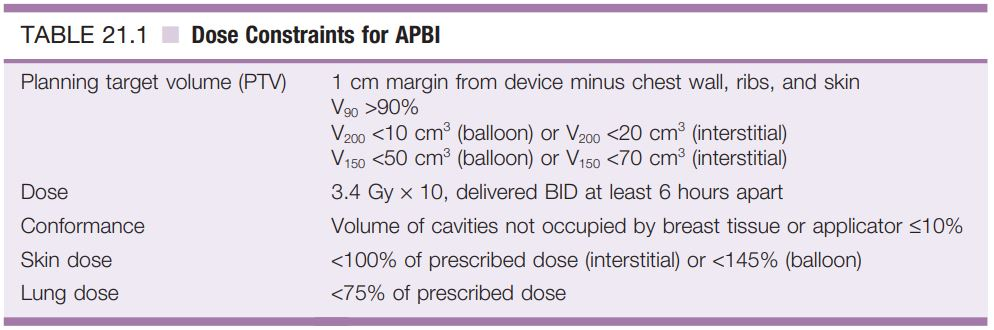
\includegraphics[width=0.8\textwidth]{Imagens/constraintsApbi.JPG}
		}%
		\caption{Constraints de Dose Para APBI}
		\label{fig:constraintsApbi}
	\end{figure}

\subsection*{Próstata}

	O implante intersticial de sementes de próstata LDR é um procedimento bem estabelecido. Os tratamentos de HDR intersticial também são usados para tratamentos de próstata, inicialmente como um boost como adjuvancia da radioterapia externa, mas cada vez mais também como terapia exclusiva.

	A justificativa para a braquiterapia de HDR para a próstata é fornecer controle local, que demonstrou ser um fator importante na resposta da doença para câncer de próstata de baixo, intermediário e alto risco. Assumindo que o modelo linear-quadrático de dose biologicamente efetiva (BED) é válido em regimes hipofracionados, pode-se argumentar que altas doses administradas em menos frações serão vantajosas para alcançar melhor controle local e, ao mesmo tempo, melhorar a preservação do tecido normal. Portanto, o escalonamento da dose combinado com o hipofracionamento tem sido o principal objetivo no desenvolvimento de novos regimes de tratamento para o câncer de próstata. A braquiterapia HDR fornece administração de uma dose localizada muito alta e gradientes de dose acentuados na direção dos órgãos de risco.

	Atualmente, a literatura sobre HDR da próstata é limitada a uma única instituição ou dados agrupados com uma ampla variedade de esquemas de fracionamento de dose. As doses prescritas  estão resumidas na \ref{fig:esquemaFracionamentoProstata}.
	
	\begin{figure}[h]
		\centering
		\fcolorbox{DarkTurquoise}{white}{%
			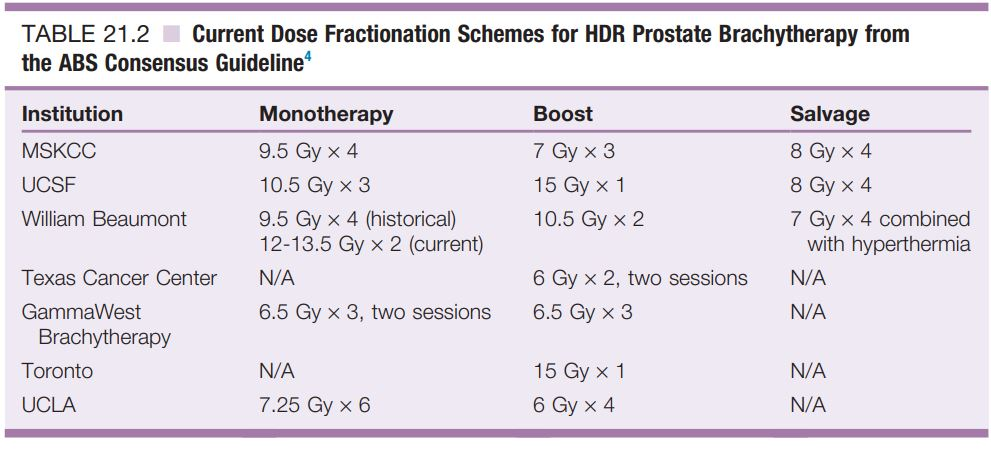
\includegraphics[width=0.8\textwidth]{Imagens/esquemaFracionamentoProstata.JPG}
		}%
		\caption{Esquemas de Fracionamento de Dose Atuais para Braquiterapia de Próstata HDR das Diretrizes de Consenso da ABS}
		\label{fig:esquemaFracionamentoProstata}
	\end{figure}

	As colocações do cateter para HDR da próstata seguem os padrões de prática estabelecidos na LDR da próstata. Os cateteres são colocados sob orientação de ultrassom transretal (TRUS); Os templates de implantes quadrados com espaçamento de agulha de 0.5 cm entre linhas e colunas são utilizados para orientar a inserção das agulhas. Dependendo do esquema de fracionamento de dose utilizado, o paciente pode ser tratado em um único dia ou internado para pernoite com anestesia peridural com os cateteres mantidos no local.

\subsection*{Outros Sítios}

	A braquiterapia intersticial também tem sido utilizada para câncer de base de língua e cabeça e pescoço, sarcomas e câncer de pulmão. A implementação da radioterapia de intensidade modulada (IMRT) para cânceres de cabeça e pescoço (H\&N), e tanto IORT quanto IMRT para tratamentos de sarcoma, reduziu a utilização de técnicas de braquiterapia intensivas em tempo e pessoal. Além disso, as técnicas mais recentes são menos invasivas, reduzindo assim o risco de eventos adversos, como infecções secundárias aos implantes intersticiais ou reações adversas aos antibióticos.

	As recomendações da ABS para braquiterapia HDR para carcinoma H\&N contêm um resumo das técnicas de implante intersticial para braquiterapia H\&N. Os cateteres são colocados o mais paralelos e equidistantes possível no plano do implante, dadas as limitações geométricas de acesso claro à base da língua ou outros locais intersticiais de H\&N. Desde a publicação dos guidelines da ABS, a técnica de IMRT foi amplamente implementada na prática clínica e substituiu amplamente a braquiterapia de H\&N.

	A braquiterapia para sarcomas é uma técnica intimamente relacionada à IORT. No momento da cirurgia, os cateteres intersticiais são suturados ao leito cirúrgico, em áreas onde margens claras não podem ser alcançadas por razões técnicas. A geometria do cateter é geralmente de plano único ou, ocasionalmente, dois planos paralelos. As recomendações da ABS para braquiterapia de sarcomas de tecidos moles recomendam a inserção do cateter de 1 a 2 cm lateralmente além do volume alvo clínico (CTV) e 2 a 5 cm além do CTV na direção longitudinal. Os pontos de entrada do cateter devem estar distantes da incisão cirúrgica, com os cateteres paralelos ou transversais na direção da incisão. Marcadores radiopacos, como clipes cirúrgicos, são usados para demarcar o CTV, bem como os órgãos de risco (OARs) nas proximidades do tumor. Os regimes de dose e fracionamento variam entre as instituições. A braquiterapia intersticial de sarcoma foi amplamente substituída por IORT ou IMRT pós-operatório.

	A braquiterapia intersticial de pulmão é realizada pela implantação de fontes radioativas no pulmão durante ressecções em cunha cirúrgicas (segmentectomia) para câncer de pulmão em estágio inicial. Fitas com sementes de \ce{^{125}I} de baixa taxa de dose fixadas em um fio de vicryl são implantadas próximas aos clipes cirúrgicos com a intenção de esterilizar possíveis margens positivas ou contaminação cirúrgica. O espaçamento dos fios pode variar de acordo com a atividade da semente ou, alternativamente, pode-se estabelecer uma faixa de atividade aceitável para espaçamento de 1 cm. O AAPM TG-222, \textit{``Operative Intersticial Lung Radiotherapy''}, é responsável por fornecer as seguintes informações:

	\begin{itemize}[label=\textcolor{CarnationPink}{$\blacktriangleright$}]
		\item Revisar as etapas do procedimento (educacional);
		\item Descrever o planejamento do tratamento e aspectos dosimétricos dos procedimentos (educacional);
		\item Recomendar parâmetros dosimétricos úteis para avaliar e especificar os tratamentos;
		\item Fazer recomendações para gerenciamento da qualidade exclusivas para os procedimentos;
		\item Recomendar uma definição para eventos médicos envolvendo esses procedimentos;
	\end{itemize}

\section{Procedimento de Implante}

\subsection*{Transporte do Paciente Durante Todo o Procedimento}

	Em muitas instalações, a localização onde ocorrerá a inserção do implante, a localização da imagem e da administração do tratamento pode não estar na mesma sala ou podem não permitir o uso da mesma mesa de tratamento. Nesses casos, o paciente precisa ser movido sem mudar a posição do implante. Vários sistemas comerciais foram desenvolvidos para auxiliar na movimentação do paciente. Eles variam de tampos de mesas deslizantes à tecnologias com suspensão.
	
	Independente da tecnologia utilizada, o implante deve ser conferido antes e depois de cada movimentação para garantir sua integridade. Especialmente para implantes geniturinários (GU) e GYN, a cama do paciente deve ser mantida plana para evitar que qualquer pressão do colchão atue nos cateteres, fazendo com que ele mude de posição ou dobre. Uma proteção é frequentemente colocada sobre os cateteres do implante se se sobressaem do paciente, de modo que esta proteção deva ter com um comprimento estendido para minimizar as chances de algo se prender em um cateter. Esta é a maior preocupação para implantes intersticiais devido ao número de cateteres envolvidos.

\subsection*{Aquisição da Imagem Para Inserção das Agulhas e Planejamento do Tratamento}

	As agulhas utilizadas em implantes intersticiais são feitas de aço cirúrgico, titânio ou plástico flexível. As agulhas de titânio são compatíveis com ressonância magnética com campo magnético de até 3 T, enquanto as agulhas de plástico são totalmente compatíveis com ressonância magnética. As agulhas de aço, embora tenham a melhor resistência mecânica, são responsáveis por criar a maioria dos artefatos nas imagens de TC. Em alguns dispositivos, uma ``caneta'' de metal central é usada para fornecer rigidez. A caneta central pode ser removida para aquisição da tomografia computadorizada, o que reduz os artefatos.

	Os implantes intersticiais, especialmente nas áreas GU/GYN, são frequentemente realizados nas proximidades de órgãos críticos. Portanto, os implantes são realizados sob orientação de imagens. Ultrassom, fluoroscopia, tomografia computadorizada e ressonância magnética podem ser utilizadas para essa finalidade, dependendo do acesso e disponibilidade dessas técnicas na instituição.

	A imagem de TC é a imagem mais utilizada para o planejamento de tratamento devido à sua disponibilidade na maioria dos departamentos de Radioterapia. A ressonância magnética (RM), se disponível, fornecerá um melhor contraste de tecidos moles em suas imagens, mas pode tornar a identificação das agulhas intersticiais mais desafiadoras do que na tomografia computadorizada (TC) devido a uma distorção geométrica causada pela RM. A fusão CT/MR pode ser utilizada para combinar as vantagens da fácil identificação do cateter, obtida nas imagens de TC, com o alto contraste de tecidos moles, disponível na RM.

	Como a ressonância magnética geralmente é realizada sem o implante estar posicionado no seu lugar, a fusão da imagem precisa ser capaz de realizar uma ``transformação não rígida''. Os erros de localização para transformações não rígidas são da ordem de vários milímetros. O report AAPM TG-132, \textit{``Use of Image Registration and Data Fusion Algorithms and Techniques in Radiotherapy Treatment Planning''}, fornece mais orientações sobre esse assunto. Alternativamente, imagens ortogonais de raios X podem ser utilizadas para planejar o tratamento de implantes intersticiais. Isso raramente é feito com o advento das imagens de TC e RM e é um método que torna difícil a avaliação nos casos de implantes com muitos cateteres ou agulhas. Além disso,  as imagens ortogonais de raios-x oferecem informações limitadas sobre os OARs.

\subsection*{Reconstrução do Catéter}

	A reconstrução precisa do cateter no conjunto de imagens de planejamento forma a base para um planejamento de tratamento preciso. Na simulação, a documentação deve ser criada para mostrar a localização do implante de agulhas no template e o esquema de numeração das agulhas desejado para os templates que não fornecem marcação do posicionamento.
	
	Para implantes sem a utilização de templates, uma foto do local do implante juntamente com a numeração desejada do cateter é uma boa ajuda visual para combinar os canais HDR com o plano de tratamento. O conjunto de imagens de planejamento deve se estender inferiormente para incluir o template das agulhas (caso tenha sido usado), para que o responsável pelo possa seguir individualmente cada agulha do template até sua ponta.

	Incertezas no matching das agulhas (posição real e imagem) são introduzidas por artefatos causados por implantes de metal ou marcadores de ouro e agulhas cruzadas. Os artefatos são maiores para agulhas de aço inoxidável e menores para cateteres de plástico. A imagem deve ser feita com os obturadores removidos. Fios fictícios flexíveis e de baixa densidade eletrônica (dummys), como fios de alumínio, podem ser usados em todos ou em alguns dos cateteres de agulha para fornecer uma ajuda na visualização.

	As incertezas devido ao cruzamento dos caminhos das agulhas dependem da elasticidade das agulhas e, portanto, são maiores para agulhas de titânio em comparação com as de aço inoxidável e podem ser bastante proeminentes para agulhas de plástico. Cateteres - especialmente aqueles que passam perto do arco púbico - às vezes são desviados por ossos ou cartilagens. Existem várias estratégias práticas para minimizar as incertezas:
	
	\begin{itemize}[label=\textcolor{CarnationPink}{$\blacktriangleright$}]
		\item Se as agulhas cruzadas puderem ser identificadas durante a simulação, um dummy pode ser inserido em uma das agulhas cruzadas para distinguir claramente os caminhos das agulhas.
		\item Se as pontas das agulhas estiverem obscurecidas por artefatos de metal, o comprimento da agulha além do template pode ser medido e, a partir disso, o comprimento da seção da agulha implantada no paciente pode ser extrapolado. Na imagem de planejamento de tratamento, geralmente é útil marcar todas as agulhas de modo que os caminhos das agulhas sejam claramente visíveis antes de trabalhar com o caminho das agulhas obscurecidas.
	\end{itemize}
	
	  A exibição de imagem 3D disponível em muitos sistemas comerciais de planejamento de tratamento (TPS) é uma excelente ajuda visual para verificar a reconstrução do cateter.

\subsection*{Controle de Qualidade dos Planos de Tratamento}

	No planejamento do tratamento, técnicas de planejamento direto ou inverso podem ser utilizadas. A braquiterapia tem maior heterogeneidade de dose do que as técnicas de teleterapia, mas o $V_{200}$ (volume que recebe 150\% da dose) deve ser limitado a áreas imediatamente adjacentes às agulhas e, idealmente, não se conectam entre as agulhas. Os esquemas de fracionamento de dose para a maioria dos alvos intersticiais variam consideravelmente entre as instituições e entre os pacientes, dependendo da situação clínica específica de cada tratamento. A verificação cuidadosa da dose prescrita em relação à diretiva escrita é, portanto, essencial para evitar possíveis erros de administração de dose.

	Como na teleterapia, uma verificação secundária e independente do plano deve ser realizada para braquiterapia intersticial. A verificação da reconstrução do cateter deve ser checada de forma independente antes do início do planejamento do tratamento para reduzir o risco de  replanejamento do paciente devido a erros cometidos nessa etapa.

	Depois que o plano for concluído e aprovado pelo médico, um duplo check completo e independente do plano deve ser realizado. Esta segunda verificação deve incluir:

	\begin{itemize}[label=\textcolor{CarnationPink}{$\blacksquare$}]
		\item Revisão da Diretiva Escrita (``prescrição escrita'');
		\item Revisão da Reconstrução do cateter, incluindo avaliação do comprimento do cateter e da distância da primeira fonte até a ponta da agulha;
		\item Verificação da correspondência da prescrição da dose com a cobertura alvo e a heterogeneidade da dose;
		\item Verificação das doses nos OARs;
		\item Verificação da correta localização dos pontos de análise de dose, se forem utilizados;
		\item Verificações secundárias da dose, utilizando software comercial ou auto-desenvolvido. Além de verificar a capacidade do sistema de planejamento de calcular a dose corretamente, ele também pode detectar quaisquer alterações feitas no plano de tratamento ocorridas entre a documentação e a verificação secundária da dose.
	\end{itemize}


\subsection*{Controles de Qualidade de Conferência Antes do Tratamento}

	O guideline ACR-ASTRO para a realização de braquiterapia HDR recomenda que, antes do início do tratamento, o médico ou o físico deve verificar, independentemente, a ordem correta das conexões do tubo de transferência da unidade de afterloader remoto para os cateteres. O comprimento de cada canal também deve ser verificado. Além disso, o físico deve verificar a transferência correta dos parâmetros de tratamento do TPS para o console do afterloader, incluindo tempos de parada, posição de parada e intensidade da fonte.

	O médico deve verificar se a posição do implante não mudou em comparação com a posição da simulação. Um método prático para fazer isso é anotar a distância da extensão do cateter além do template do implante na ficha de simulação, marcando as posições do cateter. Alternativamente, o cateter pode ser marcado onde sai da pele. Antes do início do tratamento com a fonte ativa, uma fonte dummy deve passar por todos os canais para verificar o comprimento do canal e detectar possíveis obstruções na trajetória no cateter. 
	
	A \ref{fig:checklist} mostra um exemplo de lista de verificação contendo as verificações de pré-tratamento recomendadas de acordo com o guideline ACR-ASTRO, os requisitos regulamentares do NRC e as políticas de segurança institucionais. O AAPM TG-59, com respeito a entrega de tratamento de braquiterapia HDR publicado em 1998 também fornece uma extensa lista de verificação de garantia de qualidade. Embora as seções desse relatório se refiram a tecnologias mais antigas, as recomendações gerais estão de acordo e são um pouco mais detalhadas com relação à seção de física e dos procedimentos de emergência do que o guideline ACR-ASTRO.

	\begin{figure}[h]
		\centering
		\fcolorbox{DarkTurquoise}{white}{%
			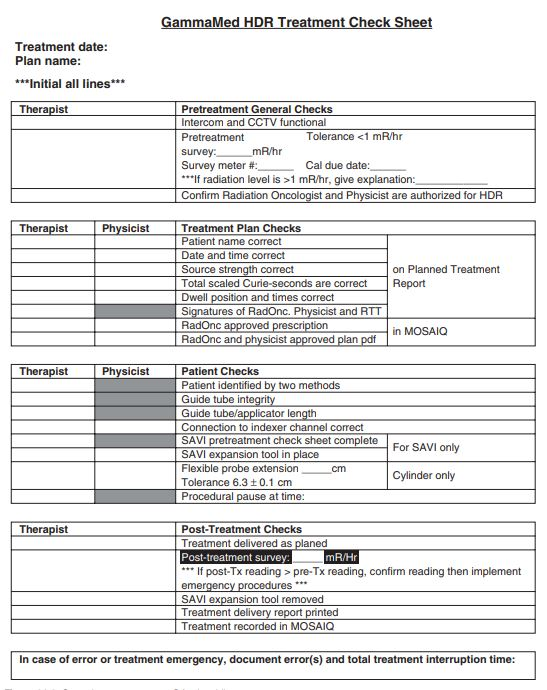
\includegraphics[width=0.8\textwidth]{Imagens/checklist.JPG}
		}%
		\caption{ChekList para implantes de braquiterapia}
		\label{fig:checklist}
	\end{figure}



\bibliography{ref.bib}
\end{document}